%!TEX root = ../a-calculus-companion.tex

\section{Integration}

%% Provide a problem where definite integration is useful,
We'll now begin to develop the concept of \emph{integration}. Where differentiation was concerned with the rate of change at a particular point, integration is concerned with the way these changes accumulate over a range of points. In order to understand this mathematically, we'll need to develop some convenient notion for dealing with sums with a large number of terms. To do this, we'll rely on Riemann sums, but first we'll introduce the ``capital sigma'' notation for sums for those who are unfamiliar.

%%% Starting with defining sum notation

Say we have numbers $a_1, a_2, a_3, a_4$, we can write their sum as $a_1+a_2+a_3+a_4$ or as $\sum_{i=1}^4a_i$ where $i$ is called the `dummy variable'. This is used to make the notation simpler and it'll reoccur often when have many terms to add together. More generally, we can write the sum of numbers $a_1, a_2,\dotsc, a_n$ as
\begin{equation}
\sum_{i=1}^{n}a_i \coloneqq a_1+a_2+\dotsb+a_n.
\end{equation}
One thing to notice is that the sum is \emph{linear}. This property is key to what follows.

\begin{lem}[Linearity of the sum]\label{LinSum}
  For any numbers $a_1, \dotsc a_n$ and $b_1, \dotsc, b_n$ and constant $c$, we have:
  \begin{enumerate}
    \item $\sum_{i=1}^{n}a_i=\sum_{i=1}^{k}a_i+\sum_{i=k+1}^{n}$ for any $k$ between $1$ and $n$,
    \item $\sum_{i=1}^{n}(a_i+b_i)=\sum_{i=1}^{n}a_i+\sum_{i=1}^{n}b_i$,
    \item $\sum_{i=1}^{n}(ca_i)=c\sum_{i=1}^{n}a_i.$
  \end{enumerate}
\end{lem}

%%%% Define linearity of \sum

This linearity also allows us to establish to the following important identities.

\begin{lem}[Formulas for Integer Sums]\label{IntegerSums}
  The following identities hold.
\begin{enumerate}
  \item $\sum_{i=1}^{n}i=\frac{n(n+1)}{2},$
  \item $\sum_{i=1}^{n}i^2=\frac{n(n+1)(2n+1)}{6},$
  \item $\sum_{i=1}^{n}i^3=\left(\frac{n(n+1)}{2} \right)^2.$
\end{enumerate}
\end{lem}
\begin{proof}
  These can be proved by induction using the linearity of the sum as established in \cref{LinSum}.
\end{proof}

\subsection{Riemann Sums}

These identities will be helpful in establishing the integrals in several of the sums that will appear. When we ``integration is concerned with the way changes accumulate'', we often want to this as the integral as the area under the curve of a function over an interval. Therefore, we start by trying to approximate this area under the curve using rectangles as in \cref{fig:RiemannSumIncresN}. In order to this, we have to divide our interval into pieces that will from the bases of these rectangles. This is the idea of the partition.
\begin{defn}[Partition]
If we have an interval $[a,b]$, we define a \emph{partition $P$ of $[a,b]$} to be the set of points $P=\{x_0,x_1,\dotsc, x_n\}$. Additionally, we define the \emph{mesh} of the partition $\abs{\abs{P}}$ to be the maximum length of the intervals $[x_i,x_{i+1}]$ in $P$.
\end{defn}

With partitions under our belt, we can define the Riemann sum: our approximation of the area underneath the curve given a particular partition.

\begin{defn}[Definition of the Riemann Sum]
  Given a function $f$ on the interval $[a,b]$ and a partition $P=\{x_0,x_1,\dotsc, x_n\}$ of [a,b], we define the \emph{upper Riemann sum of $f$ with respect to $P$} as
\begin{equation}
  U(f;P)\coloneqq\sum_{i=1}^{n}f(x_i)(x_i-x_{i-1}).
\end{equation}
Similarly, we can define the \emph{lower Riemann sum} as
\begin{equation}
  L(f;P)\coloneqq\sum_{i=1}^{n}f(x_{i-1})(x_i-x_{i-1}).
\end{equation}
Between this two, we can also define the \emph{ midpoint Riemann sum} by taking the midpoints of each interval, so that
\begin{equation}
  M(f;P)\coloneqq\sum_{i=1}^{n}f\left(\frac{x_{i}+x_{i-1}}{2}\right)(x_i-x_{i-1}).
\end{equation}
\end{defn}

\begin{figure}
\centering
\begin{subfigure}{.33\textwidth}
  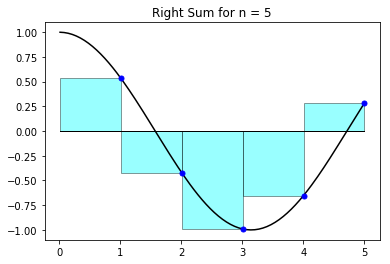
\includegraphics[width=0.9\linewidth]{RiemannSumN5.png}
  \caption{n=5}
\end{subfigure}%
\begin{subfigure}{.33\textwidth}
  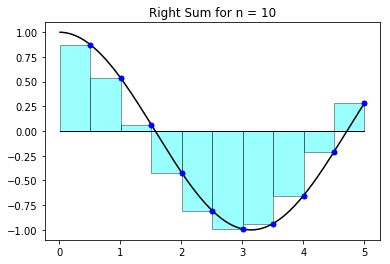
\includegraphics[width=0.9\linewidth]{RiemannSumN10.png}
  \caption{n=10}
\end{subfigure}
\begin{subfigure}{.33\textwidth}
  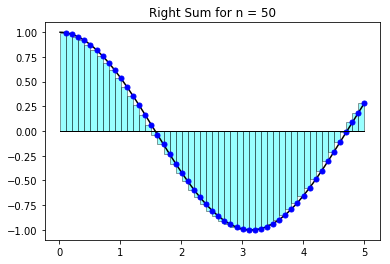
\includegraphics[width=0.9\linewidth]{RiemannSumN50.png}
  \caption{n=50}
\end{subfigure}
\caption{Upper Riemann Sums for $\cos(x)$ on $[0,5]$ using $n$ subintervals of equal length.}
\label{fig:RiemannSumIncresN}
\end{figure}


Notice each term in this sum is of the form $f(x)(x_i-x_{i-1})$, this is the area of a rectangle with height $f(x)$ and width $(x_i-x_{i-1})$. In the case of the upper sum, we take the value of $f$ at rightmost end point of the interval $[x_{i-1},x_i]$ with the left most value of the interval being used for the lower sum. If we want a function to have a definite area under it, we'd expect that the upper and lower sums fo become closer and closer as the mesh of our partition decreases since the left endpoint will approach the right endpoint of each interval. Since we'd want the intervals to be `infinitely' thin to ensure accuracy, this motivates us to define the integral in terms of limits.

\subsection{Definite Integrals}

\begin{defn}[Definition of the Definite Integral]\label{DefInt}
We define the \emph{(definite) integral of $f$ over $[a,b]$} to be
\begin{equation}
  \int_{a}^{b}f(x)dx\coloneqq \lim\limits_{\norm{P}\to 0}U(f;P)=\lim\limits_{\norm{P}\to 0}L(f;P)
\end{equation}
provided both limits exist and are equal. That is, the integral is the defined as the limit of our Riemann sum as the number of rectangles goes to infinity and each becomes infinitely thin having infinitesimal width $dx$.
\end{defn}
\begin{rem}
When the integral as defined above exists, we say that $f$ is \emph{integrable} on $[a,b]$.
\end{rem}

This raises the question of what kinds of functions are integrable for this. To provide a partial answer, we have the following proposition.
\begin{prop}\label{IntExists}
    When the function $f$ is continuous on $[a,b]$, the integral $\int_{a}^{b}f(x)dx$ exists.
\end{prop}
Though we know that every continuous function is integrable, we also know that not every function is integrable.

%% Might want to recycle this for blog post.
Notice that the limit in \cref{DefInt} is independent of partition so that if we have a sequence of partitions $P_n$ whose mesh go to 0, then we can compute the integral of $f$, so that
\begin{equation}\label{RegPartLim}
  \int_{a}^{b}f(x)dx=\lim\limits_{n\to\infty}U(f;P_n)=\lim\limits_{n\to\infty}L(f;P_n).
\end{equation}
\begin{exmp}
Suppose we want to calculate the integral of $f(x)=x^2$ on $[0,1]$. By cref{IntExists}, we can know $\int_{0}^{1}x^2dx$ exists and  pick sequence of partitions $P_n$ where each partition is given by
\begin{equation}
  P_n=\left\{0, \frac{1}{n}, \frac{2}{n},\dotsc, \frac{n-1}{n}, 1 \right\}=\left\{\frac{i}{n}\mid 0\leq i\leq n\right\},
\end{equation}
dividing $[0,1]$ into $n$ subintervals of equal length.
Since $\norm{P}$ is clearly $\frac{1}{n}$, we can write the upper Riemann sum as
\begin{equation}
  U(f;P_n)=\sum_{i=1}^{n}f\left(\frac{i}{n}\right)\left(\frac{i}{n}-\frac{i-1}{n}\right)=\sum_{i=1}^{n}\frac{i^2}{n^2}\left(\frac{1}{n}\right)=\frac{1}{n^3}\sum_{i=1}^{n}i^2.
\end{equation}
Using \cref{IntegerSums} we can reduce the above equations to
\begin{equation}
  U(f;P_n)=\frac{n(n+1)(2n+1)}{6n^3}=\frac{1}{3}+\frac{3}{n}+\frac{1}{n^2}.
\end{equation}
Taking the limit, we see that $\int_{0}^{1}x^2dx=\frac{1}{3}$ by (\ref{RegPartLim}).
\end{exmp}

This process can be visualized using computer code as in \cref{fig:RiemannSumIncresN}. Though we can use Riemann sums to solve for the integrals of simple functions directly, this method is tedious and doesn't always come easily. Therefore, we will need to develop some method of easily computing integrals, but first we must establish some more properties of the integral.

\begin{lem}[Linearity of the Integral]
The integral is linear in the following sense: For any integrable $f$ and $g$ on $[a,b]$,
\begin{enumerate}
  \item $\int_{a}^{c}f(x)dx+\int_{c}^{b}f(x)dx$ if $a<c<b$,
  \item $\int_{a}^{b}[f(x)+g(x)]dx=\int_{a}^{b}f(x)dx+\int_{a}^{b}g(x)dx$,
  \item $\int_{a}^{b}c f(x)dx=c\int_{a}^{b}f(x)dx$ for any constant $c$.
  \item $\int_{a}^af(x)dx=0$
  \item $\int_{a}^{b}f(x)dx=-\int_{b}^{a}f(x)dx$.
\end{enumerate}
\end{lem}
\begin{rem}
  Notice that the first three properties mirror those of the sum that we presented in \cref{LinSum}.
\end{rem}
A consequence of this similarity is that the sum \emph{commutes} with the integral.
\begin{cor}\label{SumIntCom}
  If $f_1, f_2, \dotsc, f_n$ are integrable functions on $[a,b]$, then
  \begin{equation}
    \int_{a}^{b}\left(\sum_{i=1}^{n}f_i(x) \right)dx= \sum_{i=1}^{n}\left(\int_{a}^{b}f_{i}(x)dx\right).
  \end{equation}
\end{cor}
We can restate \cref{SumIntCom} as ``the sum of the integral is the integral of the sum''. Furthermore, we can deduce more properties of the integral  such the integral of a non-negative function must be non-negative. With this in mind, we can get a very crude bound on the definite integral of a function.

%%%% Add other properties as exercises

\begin{prop}
  If $f$ is an integrable function on $[a,b]$ and $m$ and $M$ the minimum and maximum on $[a,b]$ respectively, then
  \begin{equation}
    m(b-a)\leq \int_{a}^{b} f(x)dx\leq M(b-a).
  \end{equation}
\end{prop}
\begin{rem}\label{ConstInt}
  This immediately tells us that for any constant function $c$ on $[a,b]$, $\int_{a}^{b} c\ dx=c(b-a)$.
\end{rem}
